% A LaTeX (non-official) template for ISAE projects reports
% Copyright (C) 2014 Damien Roque
% Version: 0.2
% Author: Damien Roque <damien.roque_AT_isae.fr>

\documentclass[a4paper,12pt]{book}
\usepackage[utf8]{inputenc}
\usepackage[T1]{fontenc}
\usepackage{float}
\usepackage[frenchb]{babel} % If you write in French
%\usepackage[english]{babel} % If you write in English
\usepackage{a4wide}
\usepackage{graphicx}
\graphicspath{{images/}}
\usepackage{subfig}
\usepackage{tikz}
\usetikzlibrary{shapes,arrows}
\usepackage{pgfplots}
\pgfplotsset{compat=newest}
\pgfplotsset{plot coordinates/math parser=false}
\newlength\figureheight
\newlength\figurewidth
\pgfkeys{/pgf/number format/.cd,
set decimal separator={,\!},
1000 sep={\,},
}
\usepackage{ifthen}
\usepackage{ifpdf}
\ifpdf
\usepackage[pdftex]{hyperref}
\else
\usepackage{hyperref}
\fi
\usepackage{color}
\hypersetup{%
colorlinks=true,
linkcolor=black,
citecolor=black,
urlcolor=black}

\renewcommand{\baselinestretch}{1.05}
\usepackage{fancyhdr}
\pagestyle{fancy}
\fancyfoot{}
\fancyhead[LE,RO]{\bfseries\thepage}
\fancyhead[RE]{\bfseries\nouppercase{\leftmark}}
\fancyhead[LO]{\bfseries\nouppercase{\rightmark}}
\setlength{\headheight}{15pt}

\let\headruleORIG\headrule
\renewcommand{\headrule}{\color{black} \headruleORIG}
\renewcommand{\headrulewidth}{1.0pt}
\usepackage{colortbl}
\arrayrulecolor{black}

\fancypagestyle{plain}{
  \fancyhead{}
  \fancyfoot[C]{\thepage}
  \renewcommand{\headrulewidth}{0pt}
}

\makeatletter
\def\@textbottom{\vskip \z@ \@plus 1pt}
\let\@texttop\relax
\makeatother

\makeatletter
\def\cleardoublepage{\clearpage\if@twoside \ifodd\c@page\else%
  \hbox{}%
  \thispagestyle{empty}%
  \newpage%
  \if@twocolumn\hbox{}\newpage\fi\fi\fi}
\makeatother

\usepackage{amsthm}
\usepackage{amssymb,amsmath,bbm}
\usepackage{array}
\usepackage{bm}
\usepackage{multirow}
\usepackage[footnote]{acronym}

\newcommand*{\SET}[1]  {\ensuremath{\mathbf{#1}}}
\newcommand*{\VEC}[1]  {\ensuremath{\boldsymbol{#1}}}
\newcommand*{\FAM}[1]  {\ensuremath{\boldsymbol{#1}}}
\newcommand*{\MAT}[1]  {\ensuremath{\boldsymbol{#1}}}
\newcommand*{\OP}[1]  {\ensuremath{\mathrm{#1}}}
\newcommand*{\NORM}[1]  {\ensuremath{\left\|#1\right\|}}
\newcommand*{\DPR}[2]  {\ensuremath{\left \langle #1,#2 \right \rangle}}
\newcommand*{\calbf}[1]  {\ensuremath{\boldsymbol{\mathcal{#1}}}}
\newcommand*{\shift}[1]  {\ensuremath{\boldsymbol{#1}}}

\newcommand{\eqdef}{\stackrel{\mathrm{def}}{=}}
\newcommand{\argmax}{\operatornamewithlimits{argmax}}
\newcommand{\argmin}{\operatornamewithlimits{argmin}}
\newcommand{\ud}{\, \mathrm{d}}
\newcommand{\vect}{\text{Vect}}
\newcommand{\sinc}{\ensuremath{\mathrm{sinc}}}
\newcommand{\esp}{\ensuremath{\mathbb{E}}}
\newcommand{\hilbert}{\ensuremath{\mathcal{H}}}
\newcommand{\fourier}{\ensuremath{\mathcal{F}}}
\newcommand{\sgn}{\text{sgn}}
\newcommand{\intTT}{\int_{-T}^{T}}
\newcommand{\intT}{\int_{-\frac{T}{2}}^{\frac{T}{2}}}
\newcommand{\intinf}{\int_{-\infty}^{+\infty}}
\newcommand{\Sh}{\ensuremath{\boldsymbol{S}}}
\newcommand{\C}{\SET{C}}
\newcommand{\R}{\SET{R}}
\newcommand{\Z}{\SET{Z}}
\newcommand{\N}{\SET{N}}
\newcommand{\K}{\SET{K}}
\newcommand{\reel}{\mathcal{R}}
\newcommand{\imag}{\mathcal{I}}
\newcommand{\cmnr}{c_{m,n}^\reel}
\newcommand{\cmni}{c_{m,n}^\imag}
\newcommand{\cnr}{c_{n}^\reel}
\newcommand{\cni}{c_{n}^\imag}
\newcommand{\tproto}{g}
\newcommand{\rproto}{\check{g}}
\newcommand{\LR}{\mathcal{L}_2(\SET{R})}
\newcommand{\LZ}{\ell_2(\SET{Z})}
\newcommand{\LZI}[1]{\ell_2(\SET{#1})}
\newcommand{\LZZ}{\ell_2(\SET{Z}^2)}
\newcommand{\diag}{\operatorname{diag}}
\newcommand{\noise}{z}
\newcommand{\Noise}{Z}
\newcommand{\filtnoise}{\zeta}
\newcommand{\tp}{g}
\newcommand{\rp}{\check{g}}
\newcommand{\TP}{G}
\newcommand{\RP}{\check{G}}
\newcommand{\dmin}{d_{\mathrm{min}}}
\newcommand{\Dmin}{D_{\mathrm{min}}}
\newcommand{\Image}{\ensuremath{\text{Im}}}
\newcommand{\Span}{\ensuremath{\text{Span}}}

\newtheoremstyle{break}
  {11pt}{11pt}%
  {\itshape}{}%
  {\bfseries}{}%
  {\newline}{}%
\theoremstyle{break}

%\theoremstyle{definition}
\newtheorem{definition}{Définition}[chapter]

%\theoremstyle{definition}
\newtheorem{theoreme}{Théorème}[chapter]

%\theoremstyle{remark}
\newtheorem{remarque}{Remarque}[chapter]

%\theoremstyle{plain}
\newtheorem{propriete}{Propriété}[chapter]
\newtheorem{exemple}{Exemple}[chapter]

\parskip=5pt
%\sloppy

\begin{document}

%%%%%%%%%%%%%%%%%%
%%% First page %%%
%%%%%%%%%%%%%%%%%%

\begin{titlepage}
\begin{center}


\includegraphics[width=0.6\textwidth]{logo_parisNanterre.png}\\[1cm]
{\large Master MIAGE}\\[0.5cm]
{\large Méthodes Informatiques Appliquées à la Gestion des Entreprises}\\[0.5cm]
{\large Promotion M1 Classique}\\[0.5cm]
{\large Année 2017-2018}\\[0.5cm]
%{\large Type de projet}\\[0.5cm]

% Title
\rule{\linewidth}{0.5mm} \\[0.4cm]
{ \huge \bfseries  Développeur au sein du portail de pilotage PPIL\\[0.4cm] }
\rule{\linewidth}{0.5mm} \\[1.5cm]
{\large Client : CNAM (Caisse Nationale de l'Assurance Maladie)}\\[0.5cm]

\includegraphics[width=0.8\textwidth]{logo-soprasteria-2.png}\\[1cm]
% Author and supervisor
\noindent
\begin{minipage}{0.4\textwidth}
  \begin{flushleft} \large
    \emph{Auteur :}\\
    M. Nicolas \textsc{Rouge}\\
  \end{flushleft}
\end{minipage}%
\begin{minipage}{0.6\textwidth}
  \begin{flushright} \large
    \emph{Tuteur entreprise :} \\
    M.~Driss \textsc{IHLALI}\\
    \emph{Tuteur MIAGE :} \\
    M.~Fabrice \textsc{LEGOND-AUBRY}
  \end{flushright}
\end{minipage}

\vfill

% Bottom of the page
{\large Version 1.3 du\\ \today}

\end{center}
\end{titlepage}

%%%%%%%%%%%%%%%%%%%%%%%%%%%%%
%%% Non-significant pages %%%
%%%%%%%%%%%%%%%%%%%%%%%%%%%%%

\frontmatter

\chapter*{Remerciements}
Je tiens à remercier toute l'équipe PPIL, avec qui j'ai travaillé au quotidien. Toute l'équipe a su m'accueillir et me donner de bons conseils, toujours avec bienveillance. 
Achref a été mon développeur référent. Il a su me donner de bons conseils et suivre ma progression au sein de mon stage. et lors de mes différentes missions de développement.
Je remercie aussi Driss pour son accueil et sa qualité d'écoute.

De nombreuses personnes ont contribué à ma bonne intégration chez Sopra Steria. Grâce notament aux réunions hebdomadaires de stagiaires. Merci à Thomas Richard pour sa présence aux réunions stagiaire, ainsi qu’à tous les stagiaires travaillant pour la CNAM au sein du pôle de Montreuil et à l'Azip.
Je remercie aussi Sara pour le suivi de mon parcours et mon intégration au sein du groupe.
Et enfin merci à toute l'équipe accueil qui a contribué à créer du dynamisme au sein du pôle.

%PPIL : Driss, Nicolas, Arkaia, Huifong, Sonia, Julie, Thomas et Marwan
%
\clearpage
\tableofcontents

\clearpage
\listoffigures

\clearpage
\chapter*{Liste des sigles et acronymes}
\begin{acronym}[CP-OFDMX] % Give the longest acronym here
\acro{BA}{\emph{Business Analyst}}
\acro{BDD}{\emph{Base De Données}}
\acro{BU}{\emph{Business Unit}}
\acro{CNAM}{\emph{Caisse Nationale d'Assurance Maladie}}
\acro{CP}{\emph{Chef de Projet}}
\acro{MEP}{\emph{Mise en producion}}
\acro{MOE}{\emph{Maitrise d’Œuvre }}
\acro{MOA}{\emph{Maitrise d’Ouvrage}}
\acro{MPD}{\emph{Modèle Physique de données}}
\acro{SFG}{\emph{Spécifications Fonctionnelles Générales}}
\acro{SFD}{\emph{ Spécifications Fonctionnelles Détaillées}}
\acro{SSG}{\emph{Sopra Steria Group}}
\acro{STD}{\emph{Spécifications Techniques Détaillées}}
\acro{V1}{\emph{Réunion hebdomadaire}}
\acro{V2}{\emph{Réunion mensuelle}}
\acro{PM}{\emph{Project Manager}}
\acro{PMO}{\emph{Project Management Office}}
\acro{SB}{\emph{Solution Builder}}
\end{acronym}

%%%%%%%%%%%%%%%%%%%%%%%%%%%%%%%%%%%%%%%%%%%%
%%% Content of the report and references %%%
%%%%%%%%%%%%%%%%%%%%%%%%%%%%%%%%%%%%%%%%%%%%

\mainmatter
\pagestyle{fancy}

\cleardoublepage

\chapter*{Introduction}
\addcontentsline{toc}{chapter}{Introduction}
\markboth{Introduction}{Introduction}
\label{chap:introduction}
%\minitoc

Sopra Steria Group m'a accueilli pour mon stage que j'ai effectué dans le cadre de ma formation MASTER 1 MIAGE. Je tenais à effectuer mon stage dans une entreprise novatrice et orienté vers le digital. Ce stage a été pour moi l'occasion d'intégrer la vie active dans le domaine qui me motive. Cela a été ma première expérience de développeur en entreprise.

Lors de ma recherche de stage, je me suis naturellement tourné vers Sopra Steria, entreprise de service numérique qui est un des leader européen de la transformation numérique.
J'ai postulé chez Sopra Steria pour la diversité des projets et des secteurs d'activités ainsi que le grand nombre de métiers. Différentes qualités que l'on retrouve chez les ESN. 

Sopra Steria Group est né de la fusion de deux SSII : Sopra et Steria en Janvier 2015.
L'entreprise intervient sur plusieurs secteurs, chaque secteur est constitué de plusieurs agences qui fonctionnent comme des entreprises indépendantes. 

A la suite d’un entretien j'ai été recruté au sein de l’une des 4 agences du Secteur public : l’agence 151 qui s’occupe du domaine "Santé, Social, Emploi".
Chaque agence est divisée en plusieurs équipes qui gèrent différents projets.

Lors de ce stage, mon objectif était de découvrir le déroulement d'un projet au sein d'une entreprise. Je suis heureux d'avoir pu intégrer une équipe. J'ai pu découvrir tous les aspects de gestion d'un projet, avec les différentes étapes, procédures et les différents rôles que chacun occupe.

J'ai intégré l'équipe PPIL qui développe un outil pour la CNAM. L'outil existe depuis 2010. Il a pour objectif, de permettre en fonction de leurs profils (par exemple Manager ou Chef de projet et bien d'autres) d'effectuer le reporting et le suivi des différents projets. 

Il est primordial de préciser que le client du projet est la CNAM, un des plus gros organisme du secteur public français. L'organisme est en pleine révolution digitale. Sopra Steria Group et ses collaborateurs l’accompagnent sur le chemin de la modernisation.

Travailler pour un client du service public a un intérêt particulier pour moi car les actions menées au quotidien par Sopra Steria ont un impact direct sur la vie de nos concitoyens.

Je suis aussi intervenu sur un projet "stagiaires" interne à Sopra Steria pour le pôle métier de l'agence 151 qui permet la gestion des compétences des différents intervenants du plateau. L'objectif principal de l'outil est de permettre aux chefs de projets ou administrateurs de projets de construire des équipes en fonction des compétences techniques des collaborateurs.

%%% Local Variables: 
%%% mode: latex
%%% TeX-master: "isae-report-template"
%%% End: 

\chapter{Contexte / Environnement}
\label{chap:premierchapitre}

Dans ce chapitre, nous allons présenter l'entreprise dans laquelle j'ai travaillé, Sopra Steria, sa structure, l'agence 151 du secteur public, ainsi que le client auquel nos développement sont destinés : la Cnam.

\section{Sopra Steria}

Sopra Steria est né de la fusion en 2014 de deux des plus anciennes Entreprises de Services du Numérique françaises, Sopra et Steria, fondées respectivement en 1968 et 1969 et marquées toutes deux par un fort esprit entrepreneurial ainsi qu'un grand sens de l’engagement collectif au service de ses clients.

Le Groupe s'affirme comme un des leaders européens de la transformation numérique.

Suite à cette fusion le groupe compte près de 42 000 collaborateurs répartis dans plus de 20 pays et a réalisé un chiffre d’affaire de 3,8 milliards d’euros en 2017.

\begin{figure}[!h]
\centering

\includegraphics[width=0.8\textwidth]{images/chiffres_cles2017.jpg}
\caption{Sopra Steria : leader européen de la transformation numérique}
\end{figure}


Sopra Steria devient alors l'un des leader Européen de la transformation numérique.

\begin{figure}[!h]
\centering
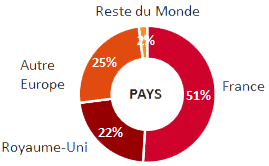
\includegraphics[width=0.5\textwidth]{images/payssoprasteria.png}
\caption{Sopra Steria : Répartition de l'activité en fonction des pays}
\end{figure}

Cette fusion a pris grâce à une forte complémentarité entre les deux entreprises : Sopra Group étant très implanté en France et peu à l'international, et Steria étant une entreprise reconnue à l'international, notamment en Europe.

//L’entreprise intervient dans de nombreux secteurs et domaines d’activité, et a du apprendre à faire face aux problèmes de managements intrinsèquement liés à sa taille et polyvalence.//

\begin{figure}[!h]
\centering
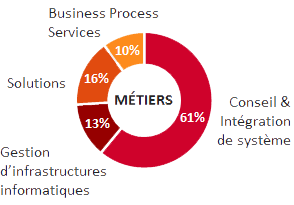
\includegraphics[width=0.5\textwidth]{images/metier_soprasteria.png}
\caption{Sopra Steria : Répartition des activités en fonction des métiers}
\end{figure}

Nous allons expliquer plus en détail les choix organisationnels de l’entreprise en prenant comme exemple notre secteur d’activité.

\section{Organisation du groupe}

//L'entreprise a choisi de diviser les secteurs d’activité et limiter le nombre d’échelons hiérarchiques au sein de chaque secteur, l’entreprise a également donné un grand pouvoir décisionnel et une grande indépendance aux collaborateurs exerçants des fonctions à responsabilités.//

La figure ci-dessous illustre la première division s’effectuant donc par secteur d’activité :

\begin{figure}[!h]
\centering
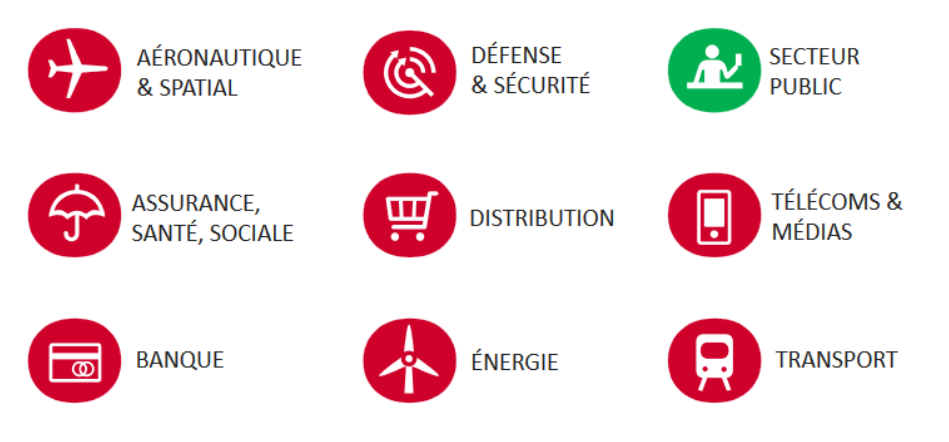
\includegraphics[width=0.8\textwidth]{images/secteurActivite.png}
\caption{Sopra Steria : Secteurs d'activités}
\end{figure}


Une Business Unit (BU) : Secteur public 
Le Secteur Public est le marché majoritaire chez Sopra Steria Group puisqu’il représente 25\% de son chiffre d’affaire.  La Business Unit du Secteur public est réparti sur 4 agences :  

\begin{itemize}
    \item Santé, Social, Emploi : Agence 151 (Sécurité sociale, Pole emploi, CNAMTS…), 
    \item echerche Enseignement : Agence 152 (ministère Éducation nationale, …), 
    \item dministration Centrale : Agence 156 (Mairie de Paris, DGFIP, ONP …), 
    \item onseil : Agence 155 (Clients transverses à toute la BU). Pour ma part, je travaille au sein de l’agence 151, pour le compte de la CNAM.
\end{itemize}


Au sein d'un même secteur d'activité, l'entreprise est divisée en agence qui fonctionnent comme des entreprises autonomes. Elles ont chacun un directeur d'agence, celui-ci dispose d'un grand pouvoir décisionnel au sein de son agence. Son objectif est que l'agence soit performante et fasse des bénéfices.
Une agence prend en charge de nombreux projets, dans notre cas, l'agence 151 gère les missions relevant du domaine de la Santé, du Social et de l’Emploi.
Ci-dessous la division au sein du secteur public.

\begin{figure}[!h]
\centering
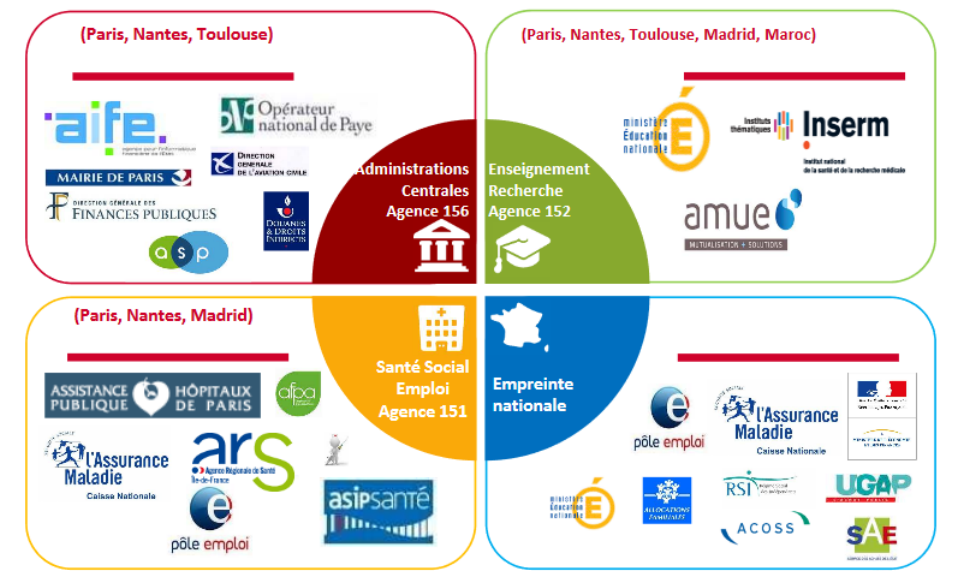
\includegraphics[width=1\textwidth]{images/divisionSecteurPublic.png}
\caption{Sopra Steria : Les agences du Secteur Public}
\end{figure}

\section{L'agence 151}

L'agence 151 est répartie dans plusieurs villes, soit dans les locaux de Sopra Steria, soit directement chez le client.

Les projets sont pris en charge par des équipes, et une équipe peut travailler sur plusieurs projets simultanément, de même plusieurs équipes peuvent travailler sur un même projet. Les équipes sont généralement d’une dizaine de membres, parmi lesquels on retrouve les rôles de :
- Chef de Projet (ou Project Manager),
- Analyste d’affaire (ou Business Analyst),
- Architecte,
- Expert produit (ou Product Expert),
- Solution Builder,
- Commercial.
Mon équipe est installée avec d'autres équipes Sopra Steria dont le client est la Cnam dans les locaux de Sopra Steria dans la tour Cytiscope à Montreuil. 

\section{Le client : la Cnam}

Chez Sopra Steria Group, plus de quatre cent collaborateurs travaillent pour le compte de la CNAM qui génère plus de 40 Millions d’euros de chiffre d’affaire. Ce chiffre est le plus important de toute la BU, ce qui fait de la CNAM un client d’importance maximale pour la société. Pour en dire un peu plus que la Caisse Nationale d’Assurance Maladie (CNAM), elle gère les branches maladie du régime général de la sécurité sociale, et représente :

\begin{itemize}
    \item 57 millions de bénéficiaires affiliés au régime général, 
    \item 4 assurés sur 5, 
    \item 75\% des dépenses de santé. 
\end{itemize}

Sopra Steria Group cherche à aider toutes ces entités en même temps dans leurs tâches quotidiennes. Les équipes de développement web (CNAMTS METIER) et de développement BI (CNAMTS BI) travaillent pour atteindre ces objectifs. Je suis moi même rattaché à la CNAM Métier. Ci-dessous la liste des projets/équipes de la CNAM Métier :

\begin{itemize}
    \item ARPEGE
    \item BIC : Briques I C
    \item CS Nantes
    \item DMP
    \item DPO
    \item DPRA
    \item INDIGO
    \item PPIL : Portail PILotage.
    \item OVERSI
\end{itemize}

\section{Le projet PPIL}
\subsubsection{Un Portail de PILotage}
PPIL permet d'assurer le suivi des projets de la CNAM.
Celui-ci répond à plusieurs besoins :
\begin{itemize}
    \item Centralisation : au sein d’un même espace des données de planification et de pilotage venant de Microsoft Project
    \item Suivi et Contrôle : vues consolidées facilitant le suivi et la vérification des données de pilotage (actualisation des données, cohérence, …)
    \item Évolutivité & Maintenance : socle permettant de mettre en place de nouvelles fonctionnalités et de les déployer pour tous les utilisateurs
    \item Communication : faciliter la diffusion de l’information
\end{itemize}
L'application PPIL a fait l'objet d'une refonte en 2017, désignée sous le nom PPIL V2. 

Les objectifs de cette version sont :
Prioritairement :
\begin{itemize}
    \item Les nouveautés concernant la gestion des projets
    \item Le fonctionnement de l’application PPIL V2 sur socle SharePoint 2013,
    \item L’iso-fonctionnalité par rapport à l’application PPIL V1, à l’exception de quelques fonctionnalités modifiées ou supprimées.
Secondairement :
    \item La simplification du portail,
    \item Des accès aux principales fonctionnalités dès la connexion en fonction des profils utilisateurs,
    \item Un usage simplifié et plus clair des fonctionnalités,
    \item La gestion des droits,
    \item La gestion des référentiels simples,
    \item La gestion des demandes et des lots.
\end{itemize}

Le Portail Pilotage est composé de différents Espaces dont l’accès est conditionné par le profil de l’utilisateur.
Les droits en lecture et/ou écriture selon le profil de l’utilisateur sont visibles dans le document de gouvernance (Gouvernance ci dessous).

Les utilisateurs accèdent à « Mon espace » et selon leurs profils, les informations restituées à l’écran varient. Les sous-espaces définis pour chaque profil suivent la description ci-après, dans l’ordre défini 

\subsubsection{Utilisateurs de PPIL :}
PPIL comprend plusieurs types de profils, on peut citer tout d'abord les profils de type opérationnel, comprenant les : 
\begin{itemize}
    \item Responsable DSI
    \item MOA
    \item Managers (Responsable de Direction ou Responsable de Département) 
    \item Chef de Projet
\end{itemize}
Et on peut citer les profils de type stratégiques, comprenant les :
\begin{itemize}
    \item PMO
    \item Responsable de domaines
\end{itemize}

Il ne faut pas oublier de citer les Visiteurs et Administrateurs.

\subsubsection{Les acteurs et leurs niveaux d'autorisation}
\begin{figure}[!h]
\centering
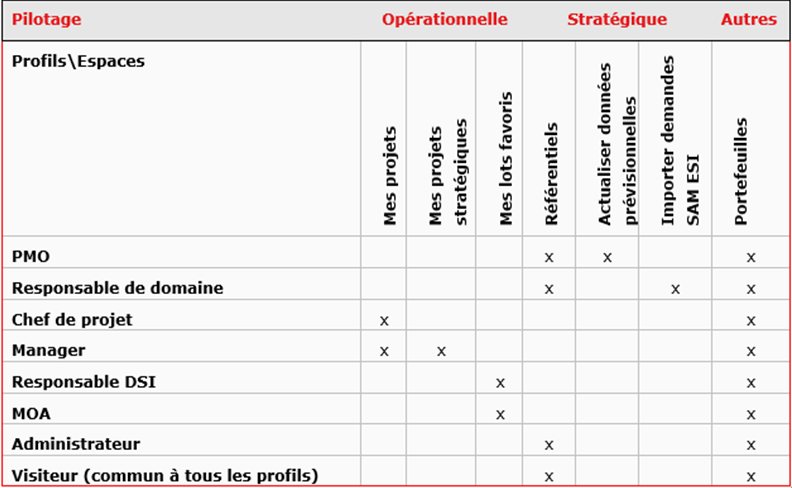
\includegraphics[width=0.8\textwidth]{images/ppil acteurs.png}
\caption{PPIL Les acteurs et leurs autorisations}
\end{figure}

\subsubsection{Lien LOT - Projet - PrtPalier}

(fig. \ref{fig:ppil lien lot projet prtpalier}).

\begin{figure}[!h]
\centering
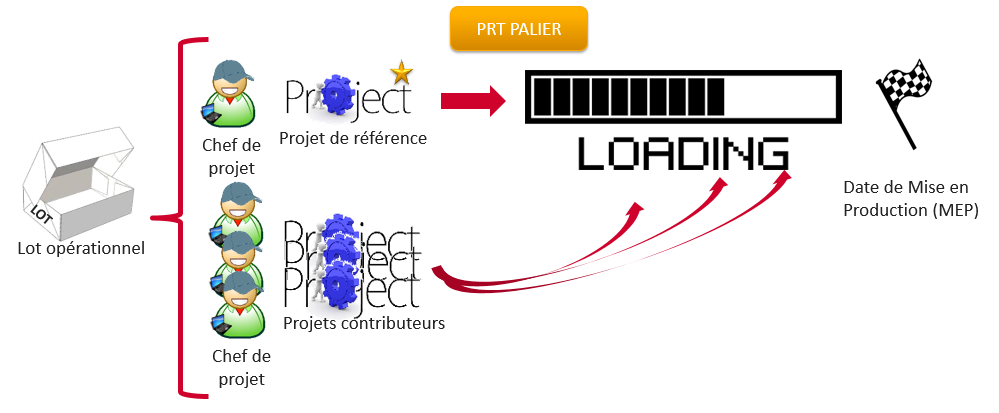
\includegraphics[width=0.9\textwidth]{images/ppil lien lot projet prtpalier.png}
\caption{PPIL lien lot projet PrtPalier}
\end{figure}

\subsubsection{Principe du Reporting - Suivi de projet}

Au sein de la CNAM, tous les acteurs d’un lot renseignent et mettent à jour le planning MSP de leur projet, en renseignant des données du type :

\vspace{1\baselineskip}

\begin{itemize}
    \item Avancement charges, 
    \item Dates des jalons, 
    \item consommé des ressources.
\end{itemize}

\vspace{1\baselineskip}

Les informations MSP sont remontées dans PPIL de plusieurs manières :
\begin{itemize}
    \item Un batch automatique lancé 2 fois par jour
    \item Dans PPIL > Données prévisionnelles
    \item Dans PPIL > Actualiser les données MSP (CP)
\end{itemize}

\vspace{1\baselineskip}

Tous les acteurs doivent renseigner les risques et problèmes rencontrés sur leur projet ainsi que l'état de leur projet (facultatif).

\subsubsection{Principe du Reporting - Exemple du CP}
Le CP du projet référent doit soumettre le reporting du lot toutes les 2 semaines (météo, tendance, situation).

Une fois soumis le reporting du lot est visible par tous les utilisateurs du PPIL.

Le Manager doit saisir la note de conjoncture du lot tous les 2 mois : 
Cette action permet d'expliquer la situation opérationnelle du lot de manière moins technique, cette note de conjoncture est plus destiné aux supérieurs hiérarchiques ( Resp DSI).

\subsubsection{Chef de Projet}

Le Dashboard du CP comprend :

\begin{itemize}
    \item Bulletin de santé
    \item Dérive des jalons
    \item Plan de charges équipe
    \item Accès à la liste de mes projets en cours
    \item Note de conjoncture à mettre à jour
    \item Alertes
    \item Rapports
\end{itemize}

Ci-dessous l'accueil du CP :

\begin{figure}[!h]
\centering
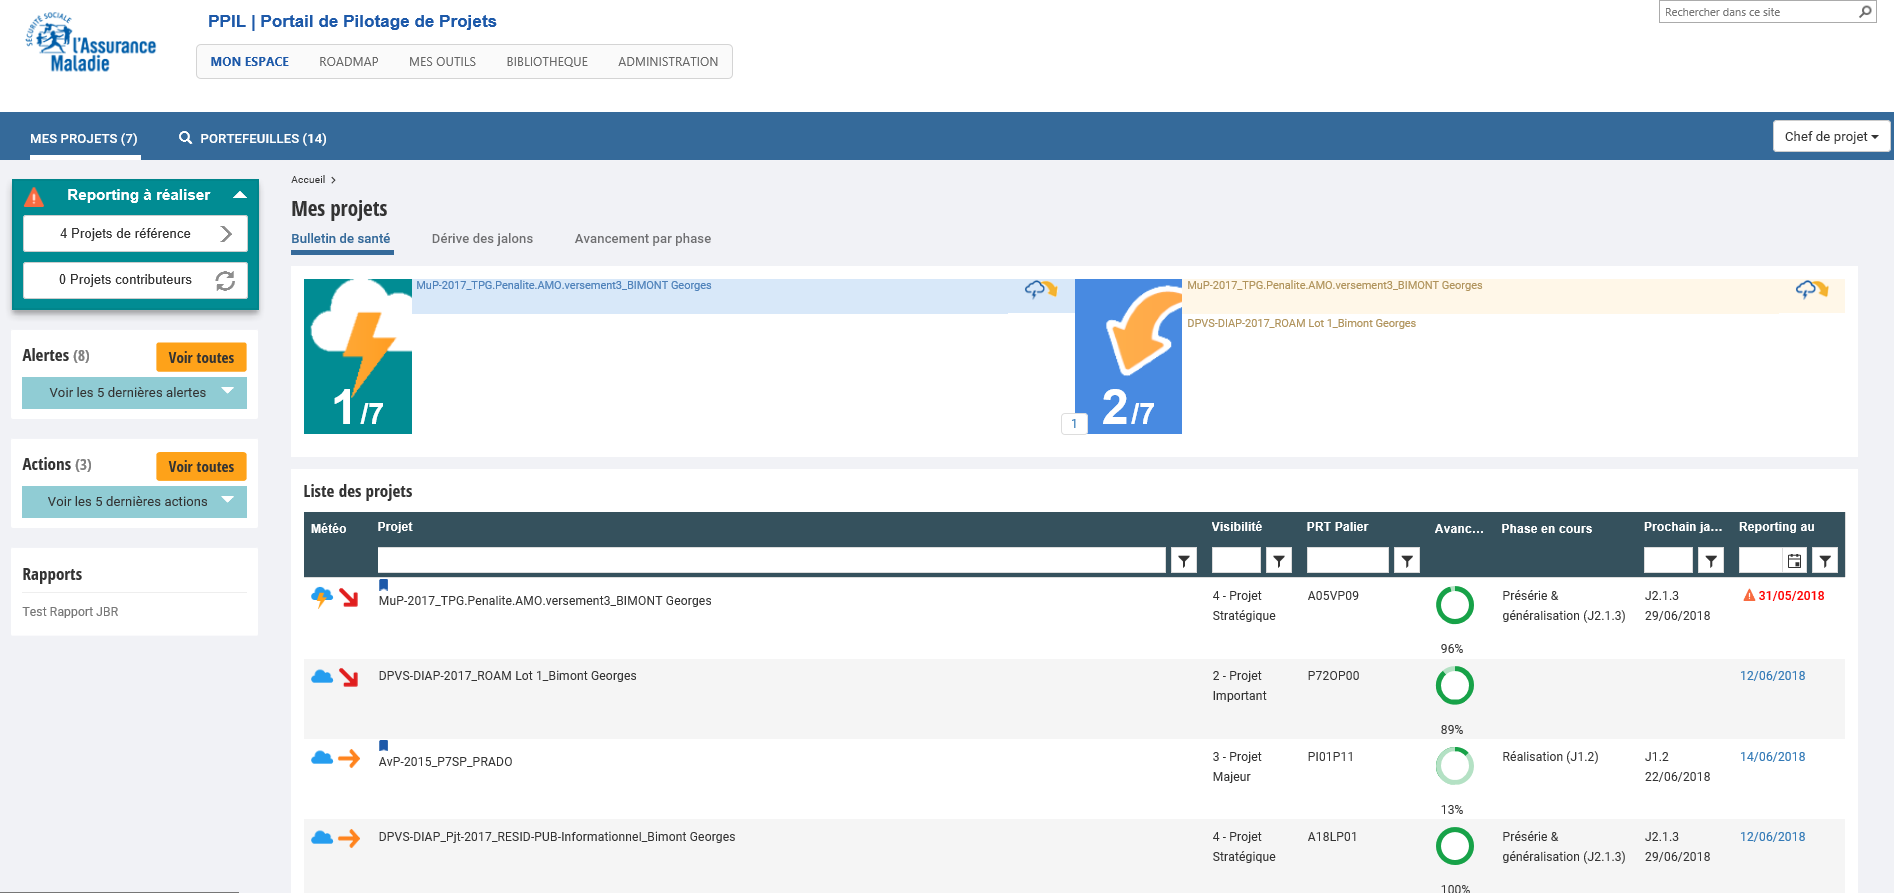
\includegraphics[width=1\textwidth]{images/ppil-CP.PNG}
\caption{PPIL : Accueil CP}
\end{figure}

Ci-dessous, un Chef de projet peut effectuer le reporting d'un projet :

\begin{figure}[!h]
\centering
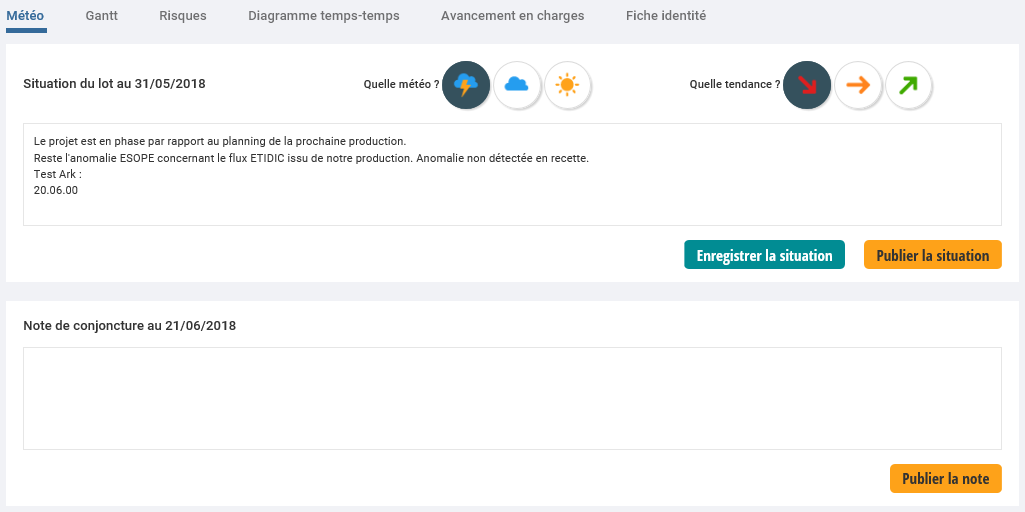
\includegraphics[width=1\textwidth]{images/ppil-meteo.PNG}
\caption{PPIL : Reporting et note de conjoncture}
\end{figure}

On peut aussi avoir accès au portail PPIL via une délégation.

%%% Local Variables: 
%%% mode: latex
%%% TeX-master: "isae-report-template"
%%% End: 
\chapter{Mon rôle au sein de PPIL}
\label{sec:unchapitre}

Au cours de mon stage, j'ai participé aux différentes phases de réalisation d'un projet : 
\begin{itemize}
    \item \textbf{phases de développement et qualification} avec le projet PPIL.
    \item \textbf{phases de conception et de cadrage} avec le projet MATRIX.
    \item \textbf{phase de relation client}, projet MATRIX.
\end{itemize}

\section{Intégrer l'équipe PPIL en participant au développement et à la qualification du projet}

Ma mission a été d'intégrer l'équipe PPIL et de participer au développement et à la qualification du projet en occupant les rôles de SB et BA. Mes objectifs de mission s'articulent autour de trois points :

\subsection{La qualification} 

Les objectifs en terme de qualification sont :
\begin{itemize}
    \item Participer à l'exécution des tests internes avec rigueur ;
    \item Remonter les anomalies détectées ;
    \item Rédiger des plans de tests ;
    \item Qualifier correctement une anomalie de manière à rendre le plus compréhensible possible l'anomalie ;
    \item Prendre en compte les retours client.
\end{itemize}

\subsection{Le développement} 

Lors du développement, je dois :

\begin{itemize}
    \item Acquérir les compétences techniques nécessaires au projet ; 
    \item Corriger les anomalies affectées par le référent technique sur le périmètre PPIL ;
    \item Garantir aucun retour bloquant en qualification interne et externe ;
    \item Garantir la non régression.
\end{itemize}

\subsection{Reporting et Autonomie}

Lors de mon stage, il est important d'être autonome dans la réalisation des tâches notamment en estimant et en respectant les délais. Il faut aussi bien s'intégrer dans l'équipe ainsi que savoir remonter les bonnes informations aux bonnes personnes. Les points que j'ai respectés sont :
\begin{itemize}
    \item Estimer ses charges, suivre son RAE, et le cas échéant expliquer les dérives ;
    \item Assurer le reporting auprès de son tuteur et remonter les difficultés rencontrées ;
\end{itemize}

\section{Fonctionnement de l'équipe}

\subsection{Les différents rôles}

J'ai intégré l'équipe de développement du Portail de PILotage (PPIL) utilisé par les chefs de projet (et autres profils) de la CNAM. L'équipe est composée de 12 collaborateurs : un chef de projet, deux référents, des développeurs (SB) et des analystes fonctionnels (BA).
Le référent technique gère la répartition et l'avancement des tâches de chacun (RAE), il est en contact permanent avec les développeurs et le chef de projet. Le référent fonctionnel est lui en contact direct avec le client, les business analystes et le chef de projet.

\subsection{Les processus mis en place}
\subsubsection{Les différents environnements}
Les BA disposent de deux environnements :
\begin{itemize}
    \item L'environnement de qualification
    \item L'environnement de test
\end{itemize}
Ils peuvent donc réaliser des tests sur deux versions différentes de PPIL simultanément. Les SB disposent de leurs propre environnement de développement. J'ai eu l'occasion de travailler sur tous ces environnements.
\subsubsection{Les processus de livraison}
A la fin d'un sprint, lorsque les développements sont terminés, le lot est livré lors d'une "livraison interne" dans l'environnement "qual" de qualification ou les BA peuvent tester la nouvelle version de PPIL. Après avoir été testé en interne, le lot est livré au client. Le client peut alors tester de son coté avec son équipe. L'étape finale est la mise en production (MEP) qui signifie que l'outil est  déployé chez le client. Les sprints durent généralement 3 semaines.
\subsubsection{Les processus au sein de l'équipe}
Au sein de l'équipe, nous nous réunissons tous les jours lors des daily-meetings, réunions de courte durée, qui permettent à chacun des membres de s'exprimer sur son avancement ou ses difficultés. Dans le cadre d'une réunion appellé V1, l'équipe se voit une fois par semaine le vendredi après-midi pendant une heure. 
Le "V1 PPIL" est constitué de :
\begin{itemize}
    \item Un point sur l'Agence 151 / plateau (le plateau contient une partie de l'agence);
    \item Un point sur PPIL ; 
    \item Une rétrospective de la semaine, santé du projet, tendance du projet, satisfaction du client ;
    \item L'évolution du projet et attribution des tâches.
\end{itemize}
%%% Local Variables: 
%%% mode: latex
%%% TeX-master: "isae-report-template"
%%% End: 
\chapter{Missions complémentaires}
\label{chap:troisiemechapitre}

\section{Le projet MATRIX}

\subsection{Contexte du projet}

En plus de ma mission principale (participer aux développement de PPIL), j'ai travaillé sur le projet MATRIX. Nous avons formé une équipe de 6 stagiaires et nous nous sommes réparti différents rôles : CP(1), RF(1), RT(1), BA(2), SB(2). Mon rôle pour ce projet est celui de SB (développeur). Nous avons tous travaillé ensemble sur les différentes phases du projet. Et surtout (pour le moment) sur les phases de relation client, cadrage et conception. Dès que nous aurons fini les phases de cadrage et conception, nous allons commencer à développer. Le temps alloué pour ce projet est d'une demi-journée minimum par semaine.
 
\subsection{Étude des besoins (phase de cadrage)}

Nous avons eu une démarche de compréhension du client. Les managers de projet ont besoin de chercher des collaborateurs en fonction des compétences de ceux-ci pour créer leurs équipes.

\subsubsection{L'importance d'étudier les outils existants}

Pour réaliser cette tâche de recherche de collaborateurs répondant à certaines compétences, les managers de projets ont des outils / processus déjà existant, tels que :

Le premier outil utilisé au niveau du pôle CNAM métier étant un fichier Excel qui répertorie les compétences des collaborateurs. Cette solution pose des difficultés principalement au niveau de la maintenabilité des informations à jour.

La deuxième solution qui s'offre aux managers de projet est, dans l'intranet du groupe (tout Sopra Steria), une section de recherche d'expert en fonction d'une compétence. Cet outil ne répertorie qu'une partie des collaborateurs (les experts dans un domaine), et la localisation de ceux-ci n'est pas à jour.

\begin{figure}[!h]
\centering
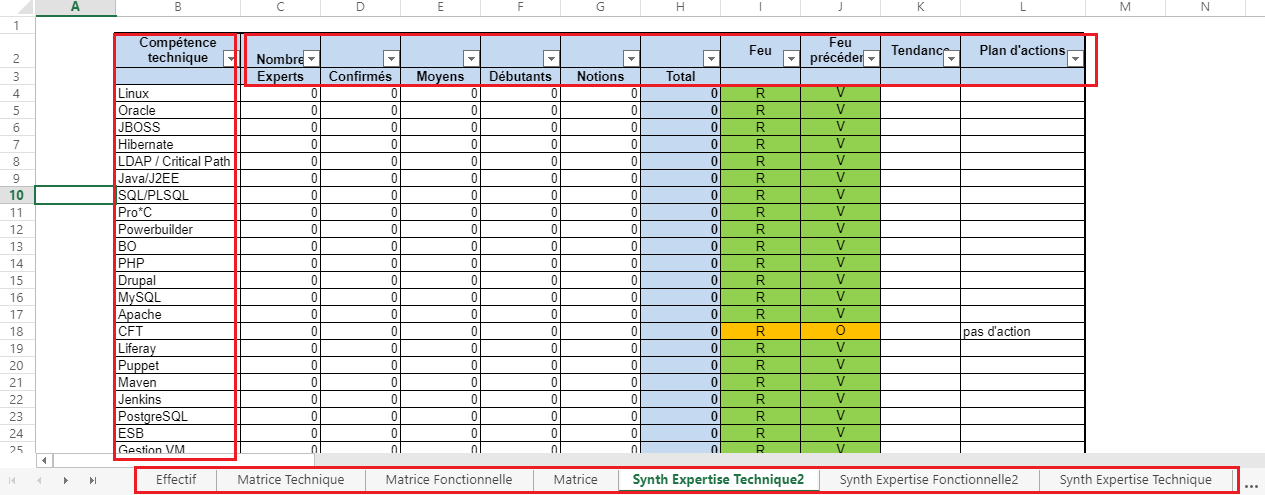
\includegraphics[width=1\textwidth]{images/MATRIX-excel.png}
\caption{MATRIX : Template du document Excel qui recense les collaborateurs en fonction de leurs compétences}
\end{figure}

Il est important d'analyser ce document car c'est celui-ci, qui dans la pratique est utilisé par les managers de projets. Pour la conception de notre application, il est important de prendre en compte la façon dont les informations sont agencées dans ce fichier Excel.

Aux vues des outils et processus cités ci-dessus, on voit bien que l'application MATRIX a sa place au sein du pôle CNAM métier et qu'elle serait un réel atout pour les managers de projets.

\subsection{Concevoir une application, notre démarche}

Lors de la conception de l'application, nous nous sommes retrouvés face à diverses problématiques. 

Par exemple, lorsque nous nous sommes demandés comment sera géré la liste des compétences en base de données : qui et comment seront ajoutées les compétences ?

Nous nous sommes retrouvés face à plusieurs questions : Est-ce qu'un utilisateur peut ajouter lui-même une fonctionnalité ? Ou bien est-ce qu'elle sont déterminées en base de données ? Si elles sont déterminées en base de données, comment en ajouter une nouvelle ? Faut-il faire des demandes administrateur ? Est-ce que les détails de la compétence (image, version) seront transmises avec ?

Toutes ces questions, nous avons pu y répondre, grâce à :
\begin{itemize}
\item l'étude des outils existants (document Excel) ;
\item différents points avec le client ;
\item priorité et faisabilité des fonctionnalités en un temps déterminé.
\end{itemize}

Nous avons choisi de :
\begin{itemize}
\item Ne pas prendre en compte les différentes versions des technologies (grâce au document Excel) ; 
\item Ne pas passer par l'administrateur pour ajouter une technologie (grâce aux entretiens avec le client) ;
\item Créer une liste par défaut des technologies en base de données (grâce au document Excel).
\end{itemize}


\subsubsection{Classer les fonctionnalités par priorité : Lot 1 et Lot 2}

Nous avons décidé que le lot 1 concernera les fonctionnalités principales et le lot 2 les fonctionnalités secondaires. Nous avons priorisé les fonctionnalités selon les besoins du client.

\subsubsection{Choix des technologies}

Nous avons été libre de choisir les technologies : 
\begin{itemize}
\item Java Spring 
\item JHipster 
\item JavaScript
\end{itemize}

Spring est un socle pour le développement d'applications très répandu en entreprise. Il représente un réel avantage en nous fournissant de nombreuses fonctionnalités qui peuvent être utilisées de plusieurs manières : ceci laisse le choix au développeur d'utiliser la solution qui correspond le plus à ses besoins.
Spring est ainsi un des frameworks le plus répandu dans le monde Java et dispose d'une grande popularité.

JHipster fournit des outils pour générer un projet avec côté client un frontal Web adaptatif (avec Angular et Bootstrap). JHipster nous permet d'atteindre nos objectif, avec plus de productivité et de qualité.

JavaScript, est le grand incontournable des pages web interactives. JHipster étant lui-même construit en parti en Angular (framework JavaScript).

\subsubsection{Mise en place des STD}

\subsubsection{Les maquettes}

Nous avons réalisé des maquettes du projet MATRIX en nous basant sur celles déjà existantes en les adaptant aux besoins du client. Ci-dessous voici deux des 7 maquettes.

\begin{figure}[!h]
\centering
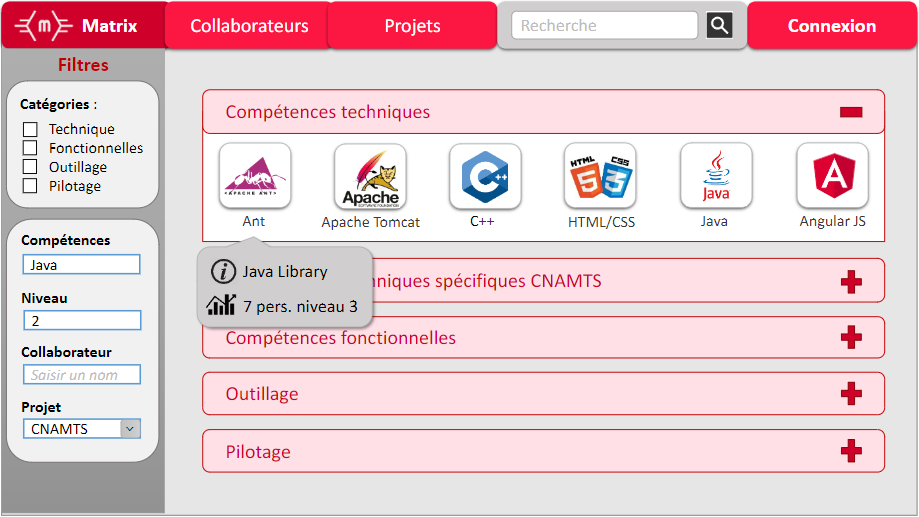
\includegraphics[width=1\textwidth]{images/matrix-maquette.png}
\caption{MATRIX : Maquette de recherche par compétence}
\end{figure}

\begin{figure}[!h]
\centering
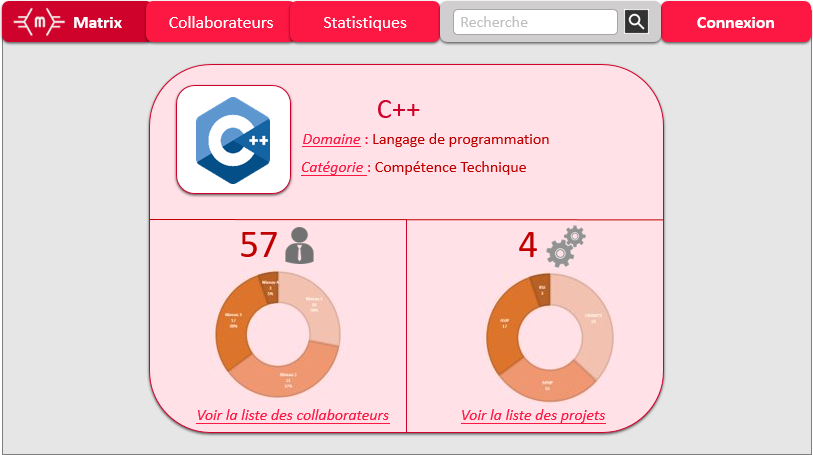
\includegraphics[width=1\textwidth]{images/matrix-maquette-competence.png}
\caption{MATRIX : Maquette détail d'une compétence}
\end{figure}

\subsubsection{La base de données}

Voici la base de données du projet :
\begin{figure}[H]
\centering
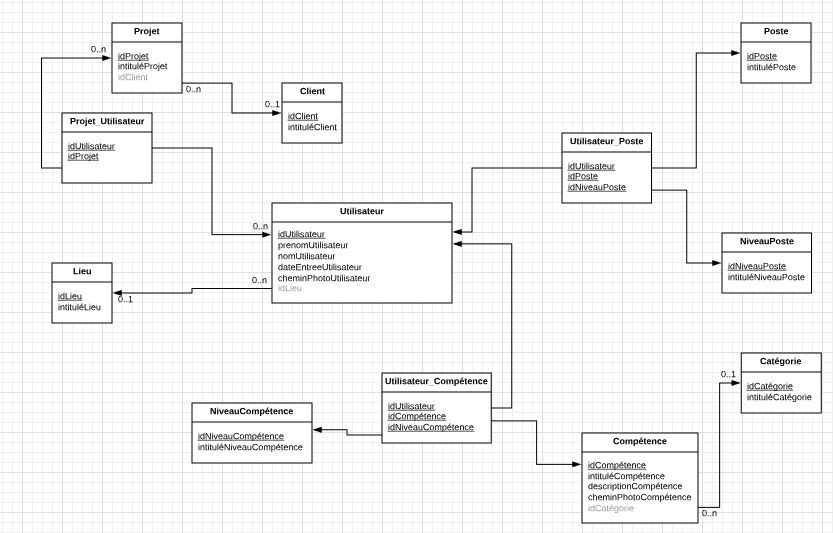
\includegraphics[width=0.8\textwidth]{images/matrix-bdd.png}
\caption{MATRIX : MCD}
\end{figure}

\subsection{Phase de développement}

\subsubsection{Installation de l’environnement}
Nous avons choisi d'utiliser l'IDE Intellij et GitLab afin de gérer nos dépots Git. Nous avons réalisé des tutoriels d'installation de nos environnements.

Nous commencerons nos développements dès que la phase de conception se terminera.

\subsection{Mise en place des SFG, STD}

Nous avons rédigé les spécifications fonctionnelles et les spécifications techniques en prenant en compte les différents lots. 

\section{Interview et présentation du métier de Business Analyste en vidéo}

Sopra Steria a proposé de réaliser une vidéo de présentation du métier de BA. Cette vidéo est destinée à présenter le métier aux nouveaux arrivants sur le pôle. Nous avons réalisé cette mission à trois. Nous avons pris l'initiative de réaliser des interview filmées de 3 collaborateurs. En parallèle, nous avons créé une animation sur l'outil Powtoon. Puis nous avons réalisé un montage vidéo en fusionnant les interview et l'animation Powtoon. Cette vidéo a été présentée à tous les acteurs du pôle Cnam Métier (plus de 100 personnes). La vidéo a été très appréciée. Cette mission a été l'occasion de découvrir le métier et d'échanger avec des collaborateurs expérimentés.

\begin{figure}[H]
\centering

\includegraphics[width=0.5\textwidth]{images/presBA.png}
\caption{Sopra Steria : Présentation du métier de BA}
\end{figure}
%%% Local Variables: 
%%% mode: latex
%%% TeX-master: "isae-report-template"
%%% End: 
\chapter{Missions complémentaires}
\label{chap:troisiemechapitre}

\section{Le projet MATRIX}

\subsection{Contexte du projet}

En plus de ma mission principale (participer aux développement de PPIL), j'ai travaillé sur le projet MATRIX. Nous avons formé une équipe de 6 stagiaires et nous nous sommes réparti différents rôles : CP(1), RF(1), RT(1), BA(2), SB(2). Mon rôle pour ce projet est celui de SB (développeur). Nous avons tous travaillé ensemble sur les différentes phases du projet. Et surtout (pour le moment) sur les phases de relation client, cadrage et conception. Dès que nous aurons fini les phases de cadrage et conception, nous allons commencer à développer. Le temps alloué pour ce projet est d'une demi-journée minimum par semaine.
 
\subsection{Étude des besoins (phase de cadrage)}

Nous avons eu une démarche de compréhension du client. Les managers de projet ont besoin de chercher des collaborateurs en fonction des compétences de ceux-ci pour créer leurs équipes.

\subsubsection{L'importance d'étudier les outils existants}

Pour réaliser cette tâche de recherche de collaborateurs répondant à certaines compétences, les managers de projets ont des outils / processus déjà existant, tels que :

Le premier outil utilisé au niveau du pôle CNAM métier étant un fichier Excel qui répertorie les compétences des collaborateurs. Cette solution pose des difficultés principalement au niveau de la maintenabilité des informations à jour.

La deuxième solution qui s'offre aux managers de projet est, dans l'intranet du groupe (tout Sopra Steria), une section de recherche d'expert en fonction d'une compétence. Cet outil ne répertorie qu'une partie des collaborateurs (les experts dans un domaine), et la localisation de ceux-ci n'est pas à jour.

\begin{figure}[!h]
\centering
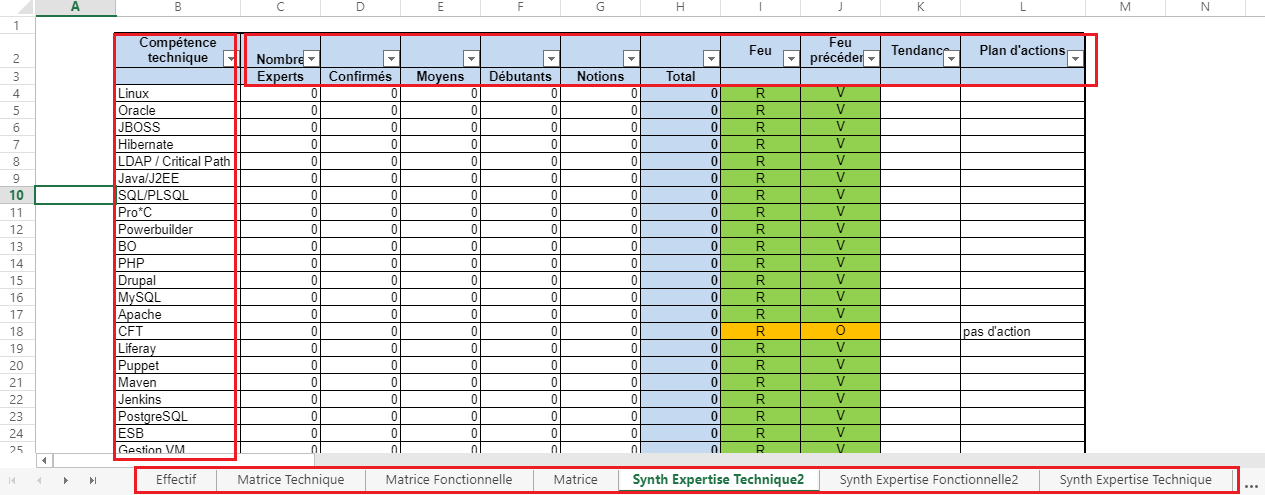
\includegraphics[width=1\textwidth]{images/MATRIX-excel.png}
\caption{MATRIX : Template du document Excel qui recense les collaborateurs en fonction de leurs compétences}
\end{figure}

Il est important d'analyser ce document car c'est celui-ci, qui dans la pratique est utilisé par les managers de projets. Pour la conception de notre application, il est important de prendre en compte la façon dont les informations sont agencées dans ce fichier Excel.

Aux vues des outils et processus cités ci-dessus, on voit bien que l'application MATRIX a sa place au sein du pôle CNAM métier et qu'elle serait un réel atout pour les managers de projets.

\subsection{Concevoir une application, notre démarche}

Lors de la conception de l'application, nous nous sommes retrouvés face à diverses problématiques. 

Par exemple, lorsque nous nous sommes demandés comment sera géré la liste des compétences en base de données : qui et comment seront ajoutées les compétences ?

Nous nous sommes retrouvés face à plusieurs questions : Est-ce qu'un utilisateur peut ajouter lui-même une fonctionnalité ? Ou bien est-ce qu'elle sont déterminées en base de données ? Si elles sont déterminées en base de données, comment en ajouter une nouvelle ? Faut-il faire des demandes administrateur ? Est-ce que les détails de la compétence (image, version) seront transmises avec ?

Toutes ces questions, nous avons pu y répondre, grâce à :
\begin{itemize}
\item l'étude des outils existants (document Excel) ;
\item différents points avec le client ;
\item priorité et faisabilité des fonctionnalités en un temps déterminé.
\end{itemize}

Nous avons choisi de :
\begin{itemize}
\item Ne pas prendre en compte les différentes versions des technologies (grâce au document Excel) ; 
\item Ne pas passer par l'administrateur pour ajouter une technologie (grâce aux entretiens avec le client) ;
\item Créer une liste par défaut des technologies en base de données (grâce au document Excel).
\end{itemize}


\subsubsection{Classer les fonctionnalités par priorité : Lot 1 et Lot 2}

Nous avons décidé que le lot 1 concernera les fonctionnalités principales et le lot 2 les fonctionnalités secondaires. Nous avons priorisé les fonctionnalités selon les besoins du client.

\subsubsection{Choix des technologies}

Nous avons été libre de choisir les technologies : 
\begin{itemize}
\item Java Spring 
\item JHipster 
\item JavaScript
\end{itemize}

Spring est un socle pour le développement d'applications très répandu en entreprise. Il représente un réel avantage en nous fournissant de nombreuses fonctionnalités qui peuvent être utilisées de plusieurs manières : ceci laisse le choix au développeur d'utiliser la solution qui correspond le plus à ses besoins.
Spring est ainsi un des frameworks le plus répandu dans le monde Java et dispose d'une grande popularité.

JHipster fournit des outils pour générer un projet avec côté client un frontal Web adaptatif (avec Angular et Bootstrap). JHipster nous permet d'atteindre nos objectif, avec plus de productivité et de qualité.

JavaScript, est le grand incontournable des pages web interactives. JHipster étant lui-même construit en parti en Angular (framework JavaScript).

\subsubsection{Mise en place des STD}

\subsubsection{Les maquettes}

Nous avons réalisé des maquettes du projet MATRIX en nous basant sur celles déjà existantes en les adaptant aux besoins du client. Ci-dessous voici deux des 7 maquettes.

\begin{figure}[!h]
\centering
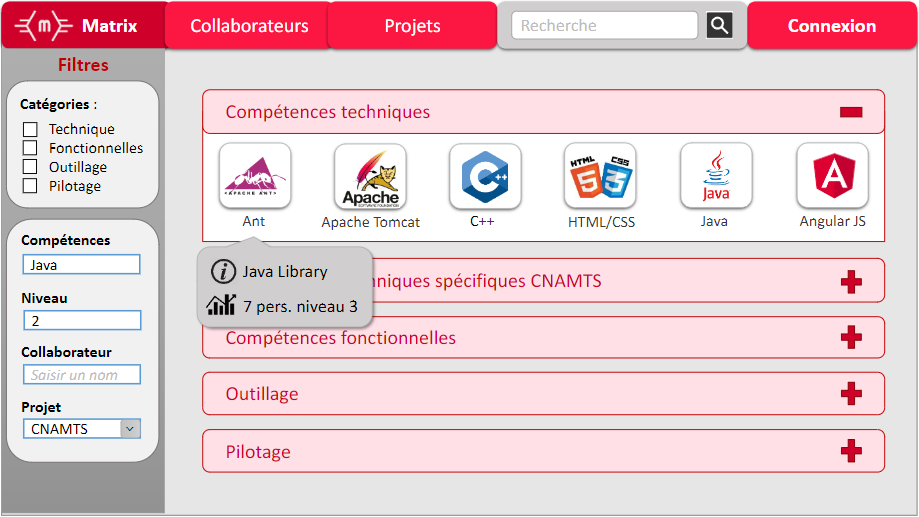
\includegraphics[width=1\textwidth]{images/matrix-maquette.png}
\caption{MATRIX : Maquette de recherche par compétence}
\end{figure}

\subsubsection{La base de données}

Voici la base de données du projet :
\begin{figure}[H]
\centering
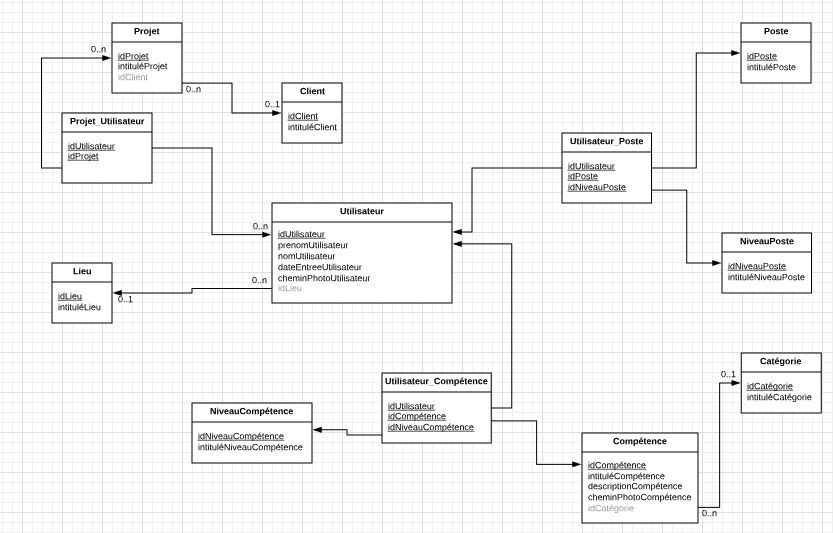
\includegraphics[width=0.8\textwidth]{images/matrix-bdd.png}
\caption{MATRIX : MCD}
\end{figure}

\subsection{Phase de développement}

\subsubsection{Installation de l’environnement}
Nous avons choisi d'utiliser l'IDE Intellij et GitLab afin de gérer nos dépots Git. Nous avons réalisé des tutoriels d'installation de nos environnements.

Nous commencerons nos développements dès que la phase de conception se terminera.

\subsection{Mise en place des SFG, STD}

Nous avons rédigé les spécifications fonctionnelles et les spécifications techniques en prenant en compte les différents lots. 

\section{Interview et présentation du métier de Business Analyste en vidéo}

Sopra Steria a proposé de réaliser une vidéo de présentation du métier de BA. Cette vidéo est destinée à présenter le métier aux nouveaux arrivants sur le pôle. Nous avons réalisé cette mission à trois. Nous avons pris l'initiative de réaliser des interview filmées de 3 collaborateurs. En parallèle, nous avons créé une animation sur l'outil Powtoon. Puis nous avons réalisé un montage vidéo en fusionnant les interview et l'animation Powtoon. Cette vidéo a été présentée à tous les acteurs du pôle CNAM Métier (plus de 100 personnes). La vidéo a été très appréciée. Cette mission a été l'occasion de découvrir le métier et d'échanger avec des collaborateurs expérimentés.

\begin{figure}[H]
\centering

\includegraphics[width=0.5\textwidth]{images/presBA.png}
\caption{Sopra Steria : Présentation du métier de BA}
\end{figure}
%%% Local Variables: 
%%% mode: latex
%%% TeX-master: "isae-report-template"
%%% End: 
\chapter*{Conclusion et perspectives}
\addcontentsline{toc}{chapter}{Conclusion}
\markboth{Conclusion}{Conclusion}
\label{sec:conclusion}

Ce rapport présente une partie du travail que j'ai réalisé au sein de Sopra Steria pendant ces deux mois de stage. J'ai beaucoup appris sur le fonctionnel du projet PPIL et les technologies utilisées pour le développement de celui-ci. J'avais pour objectif d'intégrer l'équipe PPIL et de participer à la qualification et au développement du projet. Le client est satisfait de la dernière version de PPIL qui lui a été livrée. PPIL va continuer d'évoluer avec de nouvelles fonctionnalités. A notre époque tout passe par notre smart-phone, on peut donc penser qu'une évolution mobile de restitution ou reporting des informations du portail serait la bienvenue sur mobile. J'ai également participé au cadrage et à la conception du projet MATRIX. J'entamerai les développements du projet MATRIX à partir de début juillet. 
Pour la suite de mon stage, je vais rejoindre l'équipe qui travaille sur l'application "activ'dos" afin de développer des évolutions de cette application. Une application qui possède plus de 100 000 téléchargements sur Google Play. J'ai la chance d'intégrer une équipe dynamique et motivée, de travailler sur différentes phases d'un projet et découvrir plusieurs technologies.

%%% Local Variables: 
%%% mode: latex
%%% TeX-master: "isae-report-template"
%%% End: 


\appendix
\chapter{Correction Anomalie Capacity Planning}

\begin{figure}[H]
\centering
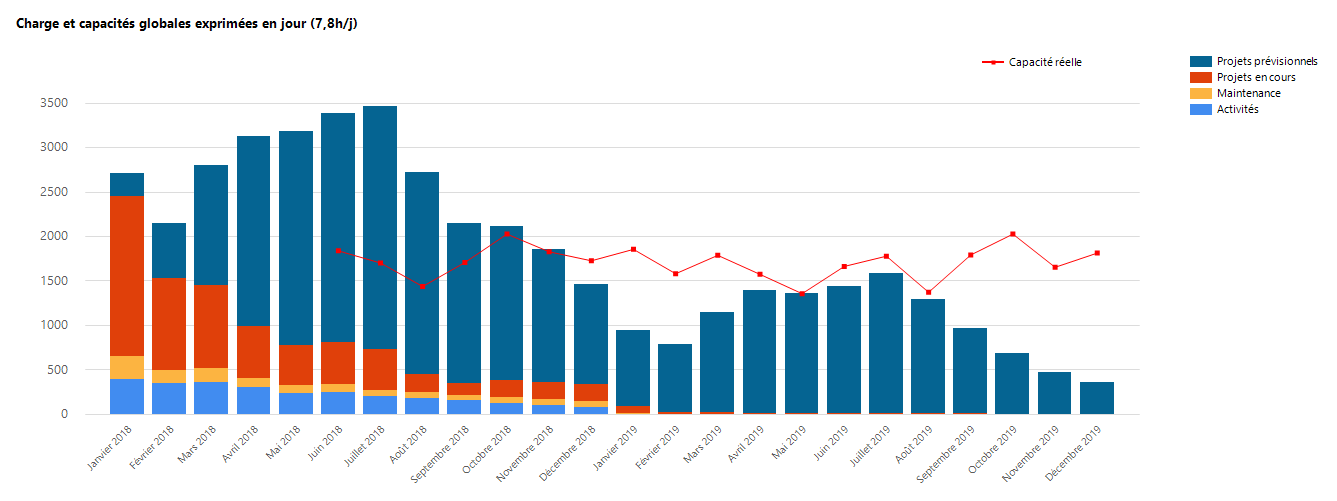
\includegraphics[width=1\textwidth]{images/capacity-planning-globales-jour.png}
\caption{La correction}
\end{figure}

\begin{figure}[H]
\centering
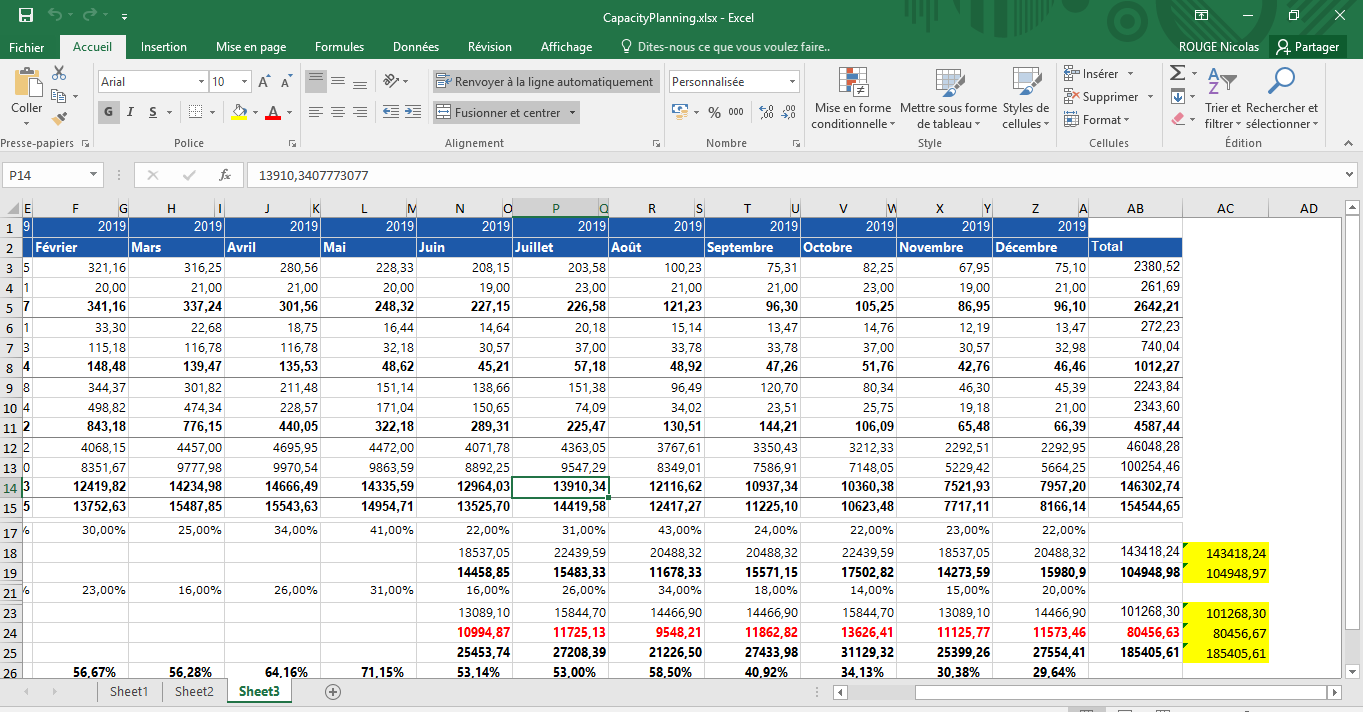
\includegraphics[width=1\textwidth]{images/excel-capacityplanning.png}
\caption{Test des données générées par ma solution}
\end{figure}

\begin{figure}[H]
\centering
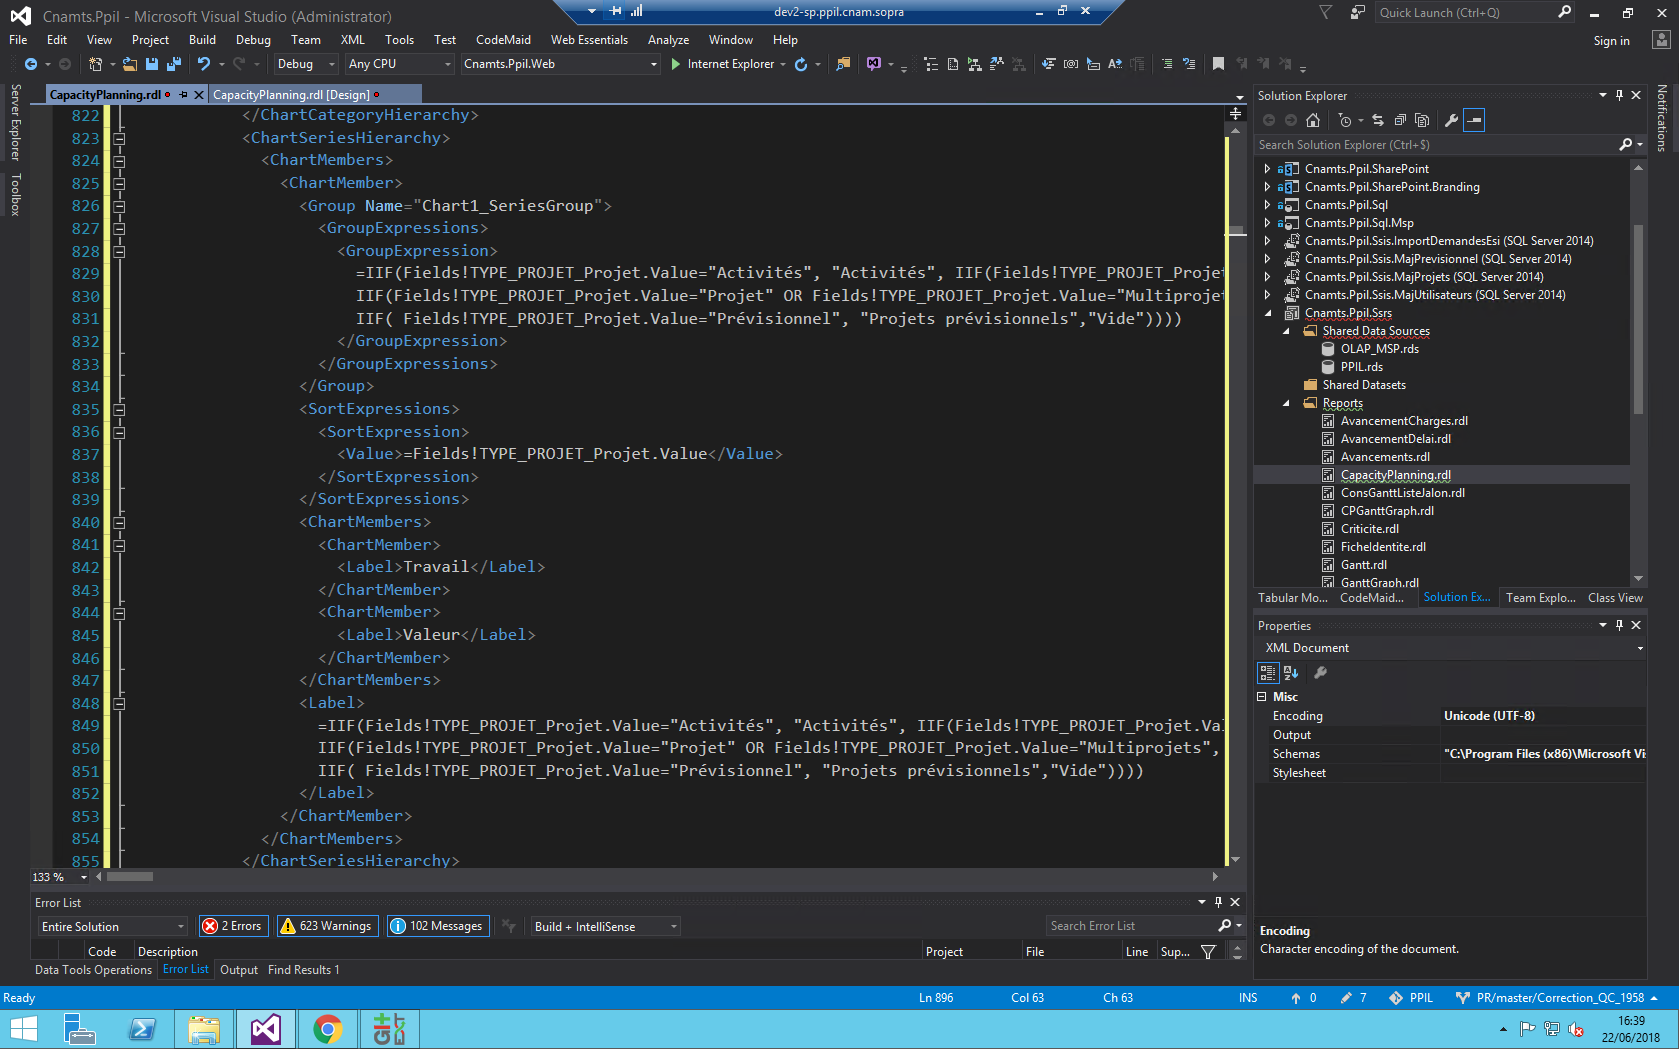
\includegraphics[width=1\textwidth]{images/env-dev.png}
\caption{Environnement de développement}
\end{figure}
\bibliographystyle{authoryear-fr}
\bibliography{references}

https://www.soprasteria.com/fr

https://assurance-maladie.ameli.fr/qui-sommes-nous/notre-fonctionnement/organisation

SFG, SFD, STD de PPIL

Manuel Utilisateur de PPIL

https://docs.microsoft.com/en-us/aspnet/mvc/overview/getting-started/introduction/adding-a-controller

https://www.telerik.com/documentation

https://www.c-sharpcorner.com/

https://www.jhipster.tech/

%\clearpage

%%%%%%%%%%%%%%%%
%%% Abstract %%%
%%%%%%%%%%%%%%%%

%\thispagestyle{empty}
%
%\vspace*{\fill}
%\noindent\rule[2pt]{\textwidth}{0.5pt}\\
%{\textbf{Résumé ---}}
%Lorem ipsum dolor sit amet, consectetur adipiscing elit. Sed non risus. Suspendisse lectus tortor, dignissim sit amet, adipiscing nec, ultricies sed, dolor. Cras elementum ultrices diam. Maecenas ligula massa, varius a, semper congue, euismod non, mi. Proin porttitor, orci nec nonummy molestie, enim est eleifend mi, non fermentum diam nisl sit amet erat. Duis semper. Duis arcu massa, scelerisque vitae, consequat in, pretium a, enim. Pellentesque congue. Ut in risus volutpat libero pharetra tempor. Cras vestibulum bibendum augue. Praesent egestas leo in pede. Praesent blandit odio eu enim. Pellentesque sed dui ut augue blandit sodales. Vestibulum ante ipsum primis in faucibus orci luctus et ultrices posuere cubilia Curae; Aliquam nibh. Mauris ac mauris sed pede pellentesque fermentum. Maecenas adipiscing ante non diam sodales hendrerit. Ut velit mauris, egestas sed, gravida nec, ornare ut, mi. Aenean ut orci vel massa suscipit pulvinar. Nulla sollicitudin. Fusce varius, ligula non tempus aliquam, nunc turpis ullamcorper nibh, in tempus sapien eros vitae ligula. Pellentesque rhoncus nunc et augue. Integer id felis.

%{\textbf{Mots clés :}}
%Lorem ipsum dolor sit amet, consectetur adipiscing elit. Sed non risus. Suspendisse lectus tortor.
\\
\noindent\rule[2pt]{\textwidth}{0.5pt}
\begin{center}
  MIAGE\\
  Université Paris Nanterre\\
  200 avenue de la République\\
  92001 Nanterre Cedex
\end{center}
\vspace*{\fill}

\end{document}